 % use the "wcp" class option for workshop and conference
 % proceedings
 %\documentclass[gray]{jmlr} % test grayscale version
 %\documentclass[tablecaption=bottom]{jmlr}% journal article
\documentclass{article} % For LaTeX2e
\usepackage{nips15submit_e,times}
\usepackage[a4paper,bindingoffset=0.2in,%
            left=1in,right=1in,top=1in,bottom=1in,%
            footskip=.25in]{geometry}

\usepackage{natbib}
\bibliographystyle{unsrtnat}

\usepackage{amsmath, amssymb}
\usepackage{mathtools}
\usepackage{algorithm, algpseudocode}

\usepackage{hyperref}
\usepackage{url}

\usepackage[titletoc,title]{appendix}

 % The following packages will be automatically loaded:
 % amsmath, amssymb, natbib, graphicx, url, algorithm2e
\newcommand\numberthis{\addtocounter{equation}{1}\tag{\theequation}}

 %\usepackage{rotating}% for sideways figures and tables
 %\usepackage{longtable}% for long tables

 % The booktabs package is used by this sample document
 % (it provides \toprule, \midrule and \bottomrule).
 % Remove the next line if you don't require it.
\usepackage{booktabs}
\usepackage{comment}
\usepackage{multirow}

% graph 
\usepackage{graphicx}
\usepackage{caption}
\usepackage{subcaption}


 % The siunitx package is used by this sample document
 % to align numbers in a column by their decimal point.
 % Remove the next line if you don't require it.
\usepackage[load-configurations=version-1]{siunitx} % newer version
 %\usepackage{siunitx}

% flow chart
\usepackage{tikz}
\usetikzlibrary{shapes.geometric, arrows}
\usetikzlibrary{bayesnet}

% attach code
\usepackage{listings}
\usepackage{adjustbox}

\definecolor{mygreen}{RGB}{28,172,0} % color values Red, Green, Blue
\definecolor{mylilas}{RGB}{170,55,241}

\lstset{language=Matlab,%
    basicstyle=\footnotesize\ttfamily,
    frame = single,
    breaklines=true,%
    morekeywords={matlab2tikz},
    keywordstyle=\color{blue},%
    morekeywords=[2]{1}, keywordstyle=[2]{\color{black}},
    identifierstyle=\color{black},%
    stringstyle=\color{mylilas},
    commentstyle=\color{mygreen},%
    showstringspaces=false,%without this there will be a symbol in the places where there is a space
    numbers=left,%
    numberstyle={\tiny \color{black}},% size of the numbers
    numbersep=9pt, % this defines how far the numbers are from the text
    emph=[1]{for,end,break},emphstyle=[1]\color{red}, %some words to emphasise
    %emph=[2]{word1,word2}, emphstyle=[2]{style},    
}


 % The optional argument of \title is used in the header
 % If you want to force a line break within the title use \titlebreak instead of \\
 % but use sparingly
\title{{\tt GURLS\_mkl}: A PFBS-based Implementation for Multiple Kernel Learning}

 % Two authors with the same address
\author{
Will Townes \\
Department of Biostatistics\\
Harvard University\\
Boston, MA 02115 \\
\texttt{ftownes@g.harvard.edu} 
\And
(Jeremiah) Zhe Liu \\
Department of Biostatistics\\
Harvard University\\
Boston, MA 02115 \\
\texttt{zhl112@mail.harvard.edu} 
}



\nipsfinalcopy
% macros from Bob Gray
\usepackage{"./macro/GrandMacros"}
\usepackage{"./macro/Macro_BIO235"}

 % Anything in the title that should appear in the main title but 
 % not in the article's header or the volume's table of
 % contents should be placed inside \titletag{}

 %\title{Title of the Article\titletag{\thanks{Some footnote}}}


 % Use \Name{Author Name} to specify the name.
 % If the surname contains spaces, enclose the surname
 % in braces, e.g. \Name{John {Smith Jones}} similarly
 % if the name has a "von" part, e.g \Name{Jane {de Winter}}.
 % If the first letter in the forenames is a diacritic
 % enclose the diacritic in braces, e.g. \Name{{\'E}louise Smith}

 % \thanks must come after \Name{...} not inside the argument for
 % example \Name{John Smith}\nametag{\thanks{A note}} NOT \Name{John
 % Smith\thanks{A note}}

 % Anything in the name that should appear in the title but not in the 
 % article's header or footer or in the volume's
 % table of contents should be placed inside \nametag{}


\begin{document}

\maketitle
\vspace*{-4em}
\tableofcontents
\thispagestyle{empty}
\newpage
\setcounter{page}{1}


%\begin{abstract}
%This is the abstract for this article.
%\end{abstract}
%\begin{keywords}
%List of keywords
%\end{keywords}


\section{Introduction}

\section{Hierarchical Dirichlet Process}


\appendix
\section{Hierarchical Dirichlet Process}

\subsection{Model}

Classic view:
\begin{alignat*}{3}
& G_0 | \gamma, H && \sim DP(\gamma, H) \\
& G_j | \alpha_0, G_0 && \sim DP(\alpha_0, G_0) \\
& \theta_{ji} | G_j && \sim G_j \\
& x_{ji} | \theta_{ji} && \sim F(\theta_{ji})
\end{alignat*}

where $P \sim DP(\alpha, G)$ adopts the stick breaking representation w.p. 1:
\begin{align*}
P &= \sum_{k=1}^\infty \pi_k \delta_{\phi_k} \qquad \mbox{where:} 
\qquad
\pi_k \sim GEM(\alpha), \quad \phi_k  \sim G
\end{align*}

Alternatively, one may describe the generative processes of $\pi_k$ and $\theta_k$ separately as:

\begin{alignat*}{3}
& \bpi_0 | \gamma && \sim GEM(\gamma) 
\qquad\qquad && \theta_k | H \sim H 
\\
& \bpi_j | \alpha_0, \bpi_0 && \sim DP(\alpha_0, \bpi_0) \\ \\
& z_{ji} | \bpi_j && \sim \bpi_j \\
& 
x_{ji} | z_{ji}, (\theta_{k})_{k=1}^\infty && \sim F(\theta_{z_{ji}})
\end{alignat*}

\begin{figure}[!h]
      \centering
\begin{subfigure}[b]{0.3\textwidth}
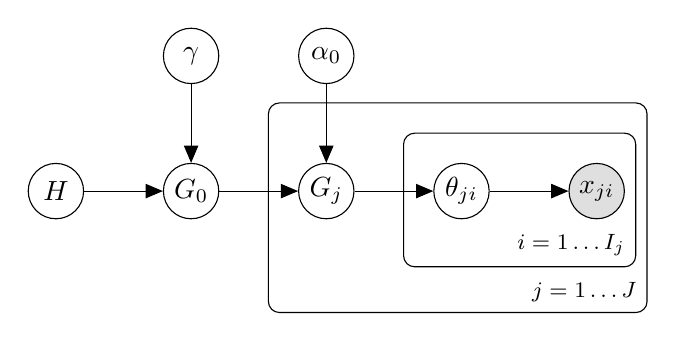
\begin{tikzpicture}[scale = 0.5]
        \node[latent] (H) {$H$} ; %
        \node[latent, right=of H] (G0) {$G_0$} ; %
        \node[latent, above=of G0] (gamma) {$\gamma$} ; %        
        \node[latent, right=of G0] (Gj) {$G_j$} ; %
        \node[latent, right=of Gj] (theta) {$\theta_{ji}$} ; %
        \node[latent, above=of Gj] (alpha) {$\alpha_0$} ; %                
        \node[obs, right=of theta] (x) {$x_{ji}$} ; %
        \plate[inner sep=0.25cm, xshift=-0.12cm, yshift=0.12cm] {plate1} {(theta) (x)} {$i = 1\dots I_j$}; %
        \plate[inner sep=0.25cm, xshift=-0.12cm, yshift=0.12cm] {plate2} {(Gj) (plate1)} {$j = 1\dots J$}; %
        \edge {H} {G0} ; %
        \edge {G0} {Gj} ; %
        \edge {Gj} {theta} ; %        
        \edge {theta} {x} ; %
        \edge {gamma} {G0} ; %
        \edge {alpha} {Gj} ; %        
\end{tikzpicture}            
\caption{Hierarchical Dirichlet Process}
\end{subfigure}

\begin{subfigure}[b]{0.3\textwidth}
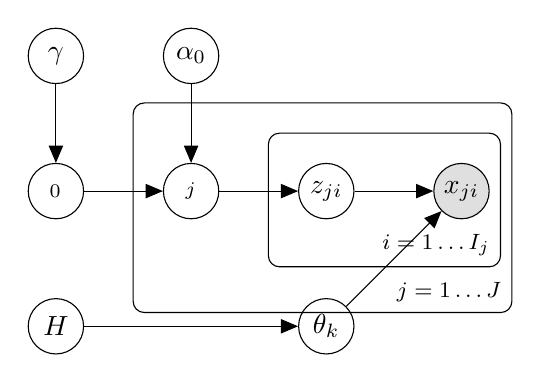
\begin{tikzpicture}[scale = 0.5]
        \node[latent] (G0) {$\bpi_0$} ; %
        \node[latent, below=of G0] (H) {$H$} ; %
        \node[latent, above=of G0] (gamma) {$\gamma$} ; %        
        \node[latent, right=of G0] (Gj) {$\bpi_j$} ; %
        \node[latent, right=of Gj] (z) {$z_{ji}$} ; %
        \node[latent, below=of z] (theta) {$\theta_{k}$} ; %                                
        \node[latent, above=of Gj] (alpha) {$\alpha_0$} ; %                
        \node[obs, right=of z] (x) {$x_{ji}$} ; %
        \plate[inner sep=0.25cm, xshift=-0.12cm, yshift=0.12cm] {plate1} {(z) (x)} {$i = 1\dots I_j$}; %
        \plate[inner sep=0.25cm, xshift=-0.12cm, yshift=0.12cm] {plate2} {(Gj) (plate1)} {$j = 1\dots J$}; %
        \edge {G0} {Gj} ; %
        \edge {Gj} {z} ; %        
        \edge {z} {x} ; %
        \edge {gamma} {G0} ; %
        \edge {alpha} {Gj} ; %        
        \edge {H} {theta} ; %                
        \edge {theta} {x} ; %       
\end{tikzpicture}      
\caption{Hierarchical Dirichlet Process}
\end{subfigure}      
      \caption{Hierarchical Dirichlet Process}
\end{figure}


\subsection{Inference}
Assuming conjugacy between $H$ and $F$ \footnote{so we can integrate out the mixture component parameters} and holding $(\gamma, \alpha_0)$ fixed, 

we now describe a simplied Gibbs approach to sample parameters $(z_{ji}, m_{jk}, \bpi_0)$ from the Chinese Restaurant Franchise (see Appendix \ref{sec:CRF}) representation of the posterior, where the parameter $z_{ji}$ are refered to respectively as customer-specific dish assignment, $m_{jk}$ as  dish-specific table count, and $\pi_0$ as global dish distribution. This particular method is  referred to as "direct assignment" in \cite{teh_hierarchical_2006} since it circumvented the issue of bookkeeping for every $t_{ij}$ (customer-specific table assignment) and $k_{jt}$ (table-specific dish assignment) variables.

In each Gibbs iteration, denote $f_k^{-x_{ji}}(x_{ji}) = 
\frac{\int f(\bx|\theta_k) h(\theta_k) d_{\theta_k}}
{\int f(\bx_{-(ji)}|\theta_k) h(\theta_k) d_{\theta_k}}$ the conditional distribution $x_{ji} | \bx_{-(ji)}$ under $\theta = \theta_k$, and assume there are currently $K$ dishes and $T$ tables, we sample $(z_{ji}, m_{jk}, \bpi_0)$ iteratively as:
\begin{enumerate}
\item Sample $z_{ji} = k | \bz_{-(ji)}, \bm, \bpi_0$ from the distribution:
\begin{align*}
z_{ji} = k | \bz_{-(ji)}, \bm, \bpi_0 \propto 
\left\{\begin{matrix*}[l]
f_k^{-x_{ji}}(x_{ji}) * (n_{jk}^{-(ji)} + \alpha_0 \pi_{0, k})  & k \leq K
\\ 
f_{K+1}^{-x_{ji}}(x_{ji}) * \alpha_0 \pi_{0, u}   & k = K+1
\end{matrix*}\right.
\end{align*}
\item Sample $m_{jk} = m | \bz, \bm_{-(jk)}, \bpi_0$, by setting $m_{jk} = \sum_{i} I(t_{ji} = t_{new}|k_{jt_{new}} = k)$,
we can sample $t_{ji}$ from:
\begin{align*}
t_{ji} = t | k_{jt} = k, \bt_{-(ji)}, \bpi_0 \propto
\left\{\begin{matrix*}[l]
n_{jt}^{-(ji)}  & t \leq T
\\ 
\alpha_0 \pi_{0, k}  & t = T+1
\end{matrix*}\right.
\end{align*}
and as in \cite{fox_bayesian_2009}, sample $I(t_{ji} = t_{new}|k_{jt_{new}} = k)$ directly from:
\begin{align*}
Bern \Big(\frac{\alpha_0 \pi_{0, k}}{n_{jk} + \alpha_0 \pi_{0, k}} \Big) 
\end{align*}

\item Sample $\bpi_0$ from distribution:
\begin{align*}
\bpi_0 & \sim Dir(m_1, \dots, m_K, \gamma)
\end{align*}
\end{enumerate}



\begin{algorithm}[H]
\caption{HDP, Gibbs Sampler through Direct Assignment}
\label{alg:MKL}
\begin{algorithmic}[1]
\Procedure{{\tt hdp\_gibbs\_ds}}{$\bK$, $\by$, $(\tau, \mu, \sigma)$}
\State $\balpha^0=\bzero$

\For{$p=1$ to ${\tt MAX\_ITER}$}
\State 
$\balpha_0^{p} = (1-\frac{\mu}{\sigma})\balpha^{p-1} - \frac{1}{\sigma n}(\bK\balpha^{p-1} - \by) $
\State 
$\balpha^p = \bS_{\frac{\tau}{\sigma}}(K, \balpha_0^{p})$
\EndFor
\State \Return $f^{\tt MAX\_ITER} = (\balpha^{\tt MAX\_ITER})^T\bk$
\EndProcedure
\end{algorithmic}
\end{algorithm}

\subsection{Application: Clustering Hierarchical Gaussian Data}
Consider mixture of Gaussian data $\bx = \{ \bx_1, \dots, \bx_K \}$ with $\bx_k \stackrel{iid}{\sim} MVN(\btheta_{k, 2 \times 1}, \bI_{2 \times 2})$ with unknown mean $\btheta$. Assuming diffused Gaussian prior $\btheta \sim N(\bzero, \sigma^2 \bI)$, the form of likelihood $F$ and base measure $H$ are:
\begin{align*}
f(x_{ji} | \btheta_k ) 
&\propto 
exp(-\frac{1}{2 \sigma^2} (x_{ji} - \btheta_k)^T(x_{ji} - \btheta_k))
\\
h(\btheta_k) 
&\propto 
exp(-\frac{1}{2\sigma_0^2}\btheta_k^T\btheta_k)
\end{align*}
Then $f_k^{-x_{ji}}(x_{ji})$ should be:
\begin{align*}
f_k^{-x_{ji}}(x_{ji}) & \sim 
N( \frac{n_{k}^{-(ji)}\sigma_0^2}{ n_{k}^{-(ji)}\sigma_0^2 + \sigma^2} 
\bar{\bx}_k^{-(ji)}, 
(1 + \frac{\sigma_0^2}{n_{k}^{-(ji)} \sigma_0^2 + \sigma^2} ) \bI)
\end{align*}


\newpage
\section{HDP for Hidden Markov Model}

\subsection{Hidden Markov Model}
\begin{figure}[!h]
      \centering
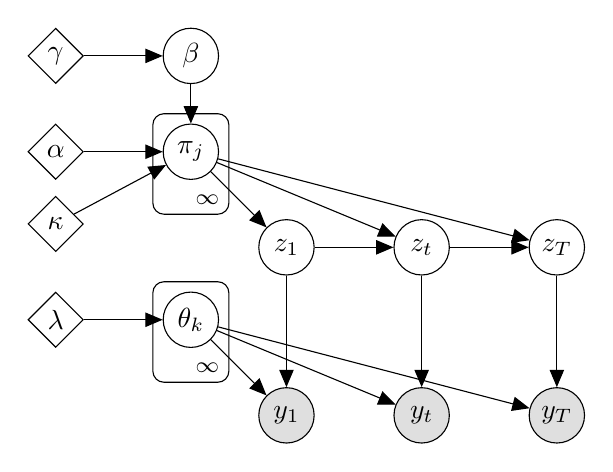
\begin{tikzpicture}[scale = 0.5]
        \node[det] (gamma) {$\gamma$} ; %
        \node[det, below = 0.5cm of gamma] (alpha) {$\alpha$}; 
        \node[det, below = 0.2cm of alpha] (kappa) {$\kappa$};       
        \node[det, below = 0.5cm of kappa] (lambda) {$\lambda$};       
        \node[latent, right = of gamma] (beta) {$\beta$} ; %                
        \node[latent, right = of alpha] (pi_j) {$\pi_j$} ; 
        \node[latent, right = of lambda] (theta_k) {$\theta_k$} ; 
        \node[latent, below right = of pi_j] (z_1) {$z_1$} ; %     
        \node[latent, right = of z_1] (z_t) {$z_t$} ; %                  
        \node[latent, right = of z_t] (z_T) {$z_T$} ; %                            
        \node[obs, below right = of theta_k] (y_1) {$y_1$} ; %     
        \node[obs, right = of y_1] (y_t) {$y_t$} ; %         
        \node[obs, right = of y_t] (y_T) {$y_T$} ; %                                  
        %
        \plate{plate_pi} {(pi_j)} {$\infty$}; %
        \plate{plate_theta} {(theta_k)} {$\infty$}; %        
		%        
        \edge {gamma} {beta} ; %       
        \edge {beta} {pi_j} ; %               
        \edge {alpha} {pi_j} ; %                       
        \edge {kappa} {pi_j} ; %                       
        \edge {lambda} {theta_k} ; %                               
        \edge {pi_j} {z_1} ; %                               
        \edge {pi_j} {z_t} ; % 
        \edge {pi_j} {z_T} ; %         
        \edge {z_1} {z_t} ; %                               
        \edge {z_t} {z_T} ; %                                       
        \edge {theta_k} {y_1} ; %                               
        \edge {theta_k} {y_t} ; % 
        \edge {theta_k} {y_T} ; %         
        \edge {z_1} {y_1} ; % 
        \edge {z_t} {y_t} ; %         
        \edge {z_T} {y_T} ; %                 
\end{tikzpicture}            
\caption{Hidden Markov Model}
\end{figure}

\begin{alignat*}{2}
& \beta | \gamma  && \sim GEM(\gamma) \\
& \pi_j | \beta, \alpha  && \sim DP(\alpha, \beta) \\
& \theta_k | H, \lambda  && \sim H(\lambda) \\
\\
& z_t | z_{t-1}, \bpi  &&\sim \pi_{z_{t-1}} \\
& y_t | z_{t}, \btheta   &&\sim F(\theta_{z_t}) \\
\end{alignat*}


\begin{align*}
f_k(y_t) &=  p(y_t | \btheta_{z_{t}}) p(z_{t}|z_{t-1}) 
\end{align*}


\subsection{Sticky HDP}
Though flexible, the fact that HDP-HMM is deploying $\pi_k \sim DP(\alpha, \beta)$ leads to:
\begin{enumerate}
\item large posterior probability for unrealistically transition dynamics
\item once instantiated, the unrealistically transition dynamics will be reinforced by CRF
\end{enumerate}
Sticky HDP address above issues by encouraging self-transition. More specifically, the base measure for $\pi_k$ is augmented \textit{a priori} from $\beta$ to:
\begin{align*}
\pi_j \sim 
DP(\alpha + \kappa, \frac{\alpha\beta + \kappa \delta_j}{\alpha + \kappa})
\end{align*}

\subsection{Inference }
Inference for HMM with Sticky HDP prior follows the sticky extension of CRF. For a observation $y_t$ at time t, "restaurant" corresponds to the state $z_t$ that $y_t$ is at, and dishes at restaurant $z_t$ indicates the potential states that $y_{t+1}$ can transit to. To improve mixing rate of state sequence $\bz$, we deploy the blocked sampler which uses a weak limit approximation of the infinite-dimension DP prior. More specifically, we assume there are $L$ states, and $\beta$ and $\pi$ follows:
\begin{align*}
\beta | \gamma & \sim Dir(\frac{\gamma}{L}, \dots, \frac{\gamma}{L}) \\
\pi_j | \alpha, \beta, \kappa & \sim 
Dir(\alpha \beta_1, \dots, \alpha \beta_j + \kappa, \dots, \alpha \beta_L)
\end{align*}

Define $\btheta_k$ as emission parameter for state $k$, we sample $(\bz, \bm, \bpi_0, \btheta)$ as follows:
 
\begin{enumerate}
\item Sample $z_{t}$ from the distribution:
\begin{align*}
z_{t} | \bz_{-(ji)}, \bm, \bpi_0, \btheta \sim f(z_t=k | \by, \bm, \bpi_0, \btheta) 
\end{align*}
where $f(z_t=k | \by)$ is calculated using the forward-backward message passing algorithm in \ref{sec:FBMP}).

\item Sample $m_{jk}$ through override correction:
\begin{enumerate}
\item Sample $m'_{jk} = \sum_{i} I(t_{ji} = t_{new}|k_{jt_{new}} = k)$, where:
\begin{align*}
I(t_{ji} = t_{new}|k_{jt_{new}} = k) & \sim 
Bern \Big(
\frac{\alpha \pi_{0, k} + \kappa \delta_j(k)}
{n_{jk} + \alpha \pi_{0, k} + \kappa \delta_j(k)} \Big) 
\end{align*}
\item Sample override variable: 
\begin{align*}
w_j & \sim 
Binom \Big(m'_{jj}, \frac{\kappa}{\kappa + \alpha\bpi_{0, j}} \Big) 
\end{align*}
\item Finally calculate $m_{jk}$ as:
\begin{align*}
m_{jk} &= 
\left\{\begin{matrix*}[l]
m'_{ij} & j \neq k
\\ 
m'_{jj} - w_j & j=k
\end{matrix*}\right.
\end{align*}
\end{enumerate}

\item Sample $\bpi_0$ from distribution:
\begin{align*}
\bpi_0 & \sim Dir(\frac{\gamma}{L} + m_1, \dots, \frac{\gamma}{L} + m_K)
\end{align*}

\item Sample $\btheta$ from distribution:
\begin{align*}
\btheta &\sim p(\btheta | \lambda, \by)
\end{align*}

\end{enumerate}


\subsubsection{Forward-backward Message Passing} \label{sec:FBMP}
The forward-backward algorithm provide an efficient method for computing node marginals $p(y_t)$. Define:
\begin{align*}
\mbox{Backward Message}: \quad & 
\beta_t(z_t) = p(\by_{T>t} | z_t)
\\
\mbox{Forward Message}: \quad &
\alpha_t(z_t) = p(\by_{T \leq t}, z_t)
\\
\mbox{Joint Message}: \quad &
\alpha_t(z_t)\beta_t(z_t) = p(\by, z_t)
\end{align*}
which can be alternatively defined using message $m_{t_1, t_2}$
\begin{align*}
\mbox{Backward Message}: \quad & 
\beta_t(z_t) = p(\by_{T>t}|z_t) = m_{t+1, t}(z_t)
\\
\mbox{Forward Message}: \quad &
\alpha_t(z_t) = p(y_t | z_t ) p(\by_{T<t}, z_t) = 
p(y_t | z_t ) m_{t-1, t}(z_t)
\end{align*}.

These two types of messages can be computed $\beta_t$ backward and $\alpha_t$ forward in time as:
\begin{alignat*}{3}
\beta_{t-1} &= \sum_{z_t} 
p(y_{t} | z_t ) && p(z_t | z_{t-1})  \beta_{t}(z_t)
\qquad \mbox{with } \quad
\beta_T(z_T) = 1
\\
\alpha_{t+1}  &=  \sum_{z_t} 
p(y_{t+1} | z_{t+1} ) && p(z_{t+1} | z_{t})  \alpha_{t}(z_t)
\qquad \mbox{with } \quad
\alpha_1(z_1) = p(y_1, z_1) = p(y_1 | z_1) \pi^0(z_1)
\end{alignat*}

Using the forward and backward messages, we can compute state assignment posterior as:
\begin{align*}
p(z_t | \by) = \frac{p(z_t, \by)}{\sum_{z_t} p(z_t, \by)} 
= 
\frac{\alpha_t(z_t)\beta_t(z_t) = p(\by, z_t)}
{\sum_{z_t} \alpha_t(z_t)\beta_t(z_t) = p(\by, z_t)} 
\end{align*}


\clearpage
\section{Chinese Restaurant Franchise}\label{sec:CRF}
A hierarchical analogy of Chinese Restaurant Process, the Chinese Restaurant Franchise offers a convenient scheme to sample from the posterior of cluster-specific $\theta$'s in HDP. This process draw below analogy:
\begin{itemize}
\item $H$ as the dish distribution for all possible dishes in the world, with the types of possible dishes being $(\theta_k)_{k=1}^\infty$.
\item  $G_0 \sim DP(\gamma, H)$ as the dish distribution for the franchise
\item $G_j \sim DP(\alpha_0, G_0)$ as the dish distribution for restaurant $j$ in the franchise
\item $\psi_{jt} \sim G_0$ as the dish served at table $t$ in restaurant $j$.\\ $k_{jt} \sim \pi_0$ as the index of dish choice for this table.
\item $\theta_{ji} \sim G_j$ as the dish will be enjoyed by customer $i$ in restaurant $j$. \\
$t_{ji} \sim \pi_j$ as the index of table choice for this customer.
\end{itemize}
Integrating over $G_j$, the sampling scheme for subject-specific dish $\theta_{ji} \sim G_j$ is:
\begin{align*}
\theta_{ji} | \btheta_{j(-i)}, \alpha_0, G_0 \sim 
\sum_{k=1}^K \frac{n_{jt.}}{\alpha_0 + n_{j..}} \delta_{\psi_{jt}} + 
\frac{\gamma}{n_{j..} + \gamma} G_0
\end{align*}
Integrating over $G_0$, the sampling scheme for table-specific dish $\psi_{jt} \sim G_0$ is:
\begin{align*}
\psi_{jk} | \Psi_{j(-k)}, \gamma, H \sim 
\sum_{k=1}^K \frac{m_{.k}}{\gamma + m_{..}} \delta_{\theta_{k}} + 
\frac{\gamma}{m_{..} + \gamma} H
\end{align*}


\clearpage
\section{References}

\bibliography{./report}



\end{document}